\documentclass[/home/greg/Thesis/main/main.tex]{subfiles}
\usepackage{floatrow}
\newfloatcommand{capbtabbox}{table}[][\FBwidth]
%\title{Neutron star mechanics in the observers inertial frame}
%\author{}

\begin{document}
\graphicspath{{/home/greg/Neutron_star_modelling/TimingResiduals/img/}}

\newcommand{\Phiexact}{\Phi_{\mathrm{exact}}}
\newcommand{\Phifit}{\Phi_{\mathrm{fit}}}
\newcommand{\wobbleangle}{\tilde{\theta}}
\FloatBarrier

\section{Timing residuals}
The principle observational quantify reported on for a pulsar is the timing 
residual. This is measured by the difference between the TOA of a pulse and
a timing model of the pulsar. It is the quasi-periodic structure in
the timing residual which we term timing-noise and hence we naturally want 
to be able to calculate the residual from our analytic models.

Using equation \eqref{eqn: Phi} we can calculate the exact phase evolution of
the star given the relevant Euler angles and components of the spin-vector; we
will label this as $\Phiexact$. Following the methods used by observers, we
take a Taylor expansion to the phase about some fixed time $t_{0}$
\begin{equation}
    \Phi(t; t_{0}, \phi, \f, \fdot, \fddot) = 
    \phi + 2\pi \left(\f(t - t_{0}) + 
                          \frac{\fdot}{2!}(t-t_{0})^{2} +
                          \frac{\fddot}{3!}(t-t_{0})^{3} 
                          \right),
\label{eqn: TR taylor expansion} 
\end{equation}
and use a least-squares fitting method to minimise the squared error between
the Taylor expansion and $\Phiexact$. The resulting coefficients $\{\phi_{0},
\f_{0}, \fdot_{0}, \fddot_{0}\}$ are the quantities best describing the NS
under a power law spindown. In pulsar astronomy these are referred to as the
timing model. We will refer to the best-fit phase as described by  these
coefficients as
\begin{equation}
    \Phifit(t) = \Phi(t; t_{0}, \phi_{0}, \f_{0}, \fdot_{0}, \fddot_{0})
\end{equation}
The phase-residual is then defined as the difference between the exact phase 
and the fitted phase
\begin{equation}
  \Delta\Phi(t) = \Phiexact(t) - \Phifit(t).
\end{equation}
It is worth noting that a phase residual depends on the fit to the entire
length of date provided in $\Phiexact$. 

The phase residual can be re-scaled to
give the timing residual by calculating the residual as a fraction of a cycle
then multiplying by the period
\begin{equation}
    \Delta T = \frac{\Delta\Phi(t)}{2\pi} P.
    \label{eqn: phase to timing}
\end{equation}
Over a typical observation periods it is possible for the period to
fractionally change due to the spindown. For this work we will report only on
phase-residuals although to make contact with observational results we will
require this re-scaling.

\subsection{Verifying the simulated timing residuals}
The effect of free-precession and the inclusion of an EM torque was
considered analytically by \citet{Jones2001}. They calculated several useful
results for the magnitude of variations in the residual; we can use these to
verify our simulations. By simulating the residuals directly, we can improve
on their results by understanding some of the more subtle features.

\subsection{Understanding the wobble angle}
The analytic calculations of \citet{Jones2001} are based on the wobble angle 
$\wobbleangle$ which the spin-vector makes with the axis about which it precesses.
This axis depends on the mass distribution, and any applied torques. Before
continuing we discuss what this wobble angle is given by in different cases.

To understand the wobble angle we refer to figure \ref{fig: reference plane}
illustrating the so-called reference plane from \citet{Jones2001}
\begin{figure}
    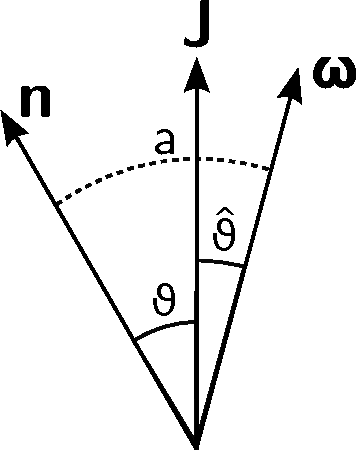
\includegraphics[width=0.2\textwidth]{/home/greg/Neutron_star_modelling/Illustrations/ReferencePlane/ReferencePlane.pdf}
    \caption{The reference plane containing the angular momentum vector $\spin$,
    the angular momentum vector $\L$ and the symmetry axis $n$ lying along the
    body-frame $\z$ axis. The dotted line indicates the polar angle $a$ between
    the body-frame $\z$ axis and the spin vector.}
    \label{fig: reference plane}
\end{figure}
This reference plane is a direct result of the relation 
\begin{align}
    L_{a} = I_{ab} \omega_{b} &&& I_{ab} = I_{0} \delta_{ab} + \epsI\delta_{3a}\delta_{3b}
\end{align}
since $\mathbf{n}$ lies along the $\z$ axis of the body frame. It was shown by
\citet{Jones2001} that for nearly spherical bodies
\begin{equation}
    \hat{\theta} \approx \epsI \sin\theta \cos\theta.
\end{equation}
Taking also the limit that $\theta \ll 1$ it can be shown that
\begin{equation}
    \hat{\theta} \approx \epsI \theta
\end{equation}
and so when comparing the two angles $\hat{\theta} \ll \theta$ such that 
$a\approx \theta$.

For a biaxial body free of torques, the spin vector precesses about the
symmetry axis of the moment of inertia $\mathbf{n}$. Using the approximations
mentioned above then the wobble angle is given by
\begin{equation}
    \wobbleangle \approx \theta.
\end{equation}
Therefore, solutions without precession correspond to $a=0$.
%For triaxial bodies it can precess
%about either of the stable axis of the moment of inertia \citep{Landau1969}. 

Including the EM torque from equation \eqref{eqn: torque} introduces two effects:
the first and the largest is the transformation induced by the anomalous torque
which causes the spin-vector to precess about the principle axis of an
\emph{effective} body-frame. This has already been discussed in chapter \ref{sec:
effective body frame} and results in a wobble angle
\begin{equation}
    \wobbleangle \approx \theta - \beta
    \label{eqn: wobble angle no SD}
\end{equation}
where $\beta$ is the rotation from the body-frame to the effective body-frame.
In this case non-precessing solutions correspond to $a \approx \beta$.

The second, smaller effect is that, even without the anomalous torque the spin-down 
torque introduces a time-varying component to the angular momentum vector. Which
will change the axis of precession. The magnitude of this time
varying component is given by 
\begin{equation}
|\dot{\L}| \sim L \omega \hat{\theta}
\end{equation} 
this can be equated to the magnitude of the spindown torque
\begin{equation}
|T_{\mathrm{sd}}| = I_{0}|\dot{\spin}|
\end{equation}
rearranging for the angle between the spin-vector and angular momentum yeilds
\begin{equation}
    \hat{\theta} = \frac{I_{0}\dot{\omega}}{I \omega^{2}} = \frac{P}{\tauS}
\end{equation}
The wobble angle due to this spin-down torque is then given by 
\begin{align}
    \wobbleangle_{\mathrm{SD}} & = \theta + \hat{\theta}\\
                 & = \hat{\theta}\left(1 + \frac{1}{\epsI}\right) \\
                 & = \frac{P}{\tauS}\left(1 + \frac{1}{\epsI}\right) \\
                 & \approx \frac{P}{\tauS}{\frac{1}{\epsI}}
    \label{eqn: spindown wobble angle}
\end{align}
Therefore we can write the wobble angle in general as
\begin{equation}
    \wobbleangle = \theta - \beta + \frac{P}{\tauS}\frac{1}{\epsI}
    \label{eqn: wobble angle}
\end{equation}
Now for solutions where the precession is important the final term
will be negligable and so we generally refer to equation \eqref{eqn: wobble angle no SD}.
However, when we set up initial conditions to minimise the precession: either
$a_{0}=0$ for free precession or $a_{0} = \beta$ when incuding the anomalous
torque; the approximations we made earlier become important. Now the wobble angle
due to the spindown can dominate and so we should use the full expression in
equation \eqref{eqn: wobble angle}.


\subsubsection{Effect of free precession on the phase residual: geometric effect}
\citet{Jones2001} analysed the geometric effect that precession will have on
the timing residual. This was done by considering the motion of the magnetic
dipole in the inertial frame as the superposition of motions due to the fast
rotation period and the slow precession. The results
must be separated into two cases when $\theta > \chi$ and $\theta < \chi$. Of
these two the authors argue that `the wobble angle  of rapidly rotating
stars are limited to small values by the finite crustal breaking strain'. Therefore, 
the second case $\theta < \chi$ holds greater physical relevance and so we 
focus on this region of parameter space. The phase residual for such NSs was 
shown to be given by  
\begin{equation}
    \Delta\Phi^{49}(t) = -\wobbleangle \cot\chi\cos(\dot{\psi t}),
    \label{eqn: Jones 49}
\end{equation}
where the superscript here refers to the equation number from \citet{Jones2001}.
For a freely precession star $\dot{\psi}=\epsI \f$ is the constant free
precession frequency. Therefore, the magnitude of variations is given by 
$|\Delta\Phi^{49}|=\wobbleangle \cot(\chi)$. 

Equation \eqref{eqn: Jones 49} is calculated in the absence of any EM torque.
Nevertheless, it is still appropriate when such a torque is applied provided
that the geometric effect is stronger that any other (these are discussed in
the next few sections). As such we begin by simulating a NS with the properties
listed in table \ref{tab: 49 verification properties}. Nonphysical values of the
rotation frequency and magnetic field have been used to aid the computational
speed. The resulting phase residual, in cycles, is given in figure \ref{fig:
PR 49}.

%\begin{table}[ht]
    %\centering
    % \begin{tabular}{ccl}
\multicolumn{3}{c}{Simulation parameters} \\
\hline
$\omega_0$  &=& 15.5 rad/s\\
$B_0$  &=& $ 1.581\times 10^{14} $ G \\
$\chi$  &=& 49.99$^{\circ}$ \\
$a_0$ &=& 2.00$^{\circ}$ \\
$\tilde{\theta}$ &= & 2.04$^{\circ}$
\end{tabular}
    
    %\caption{}
    %\label{tab: 49 verification properties}
%\end{table}

%\begin{figure}[ht]
%\centering
	%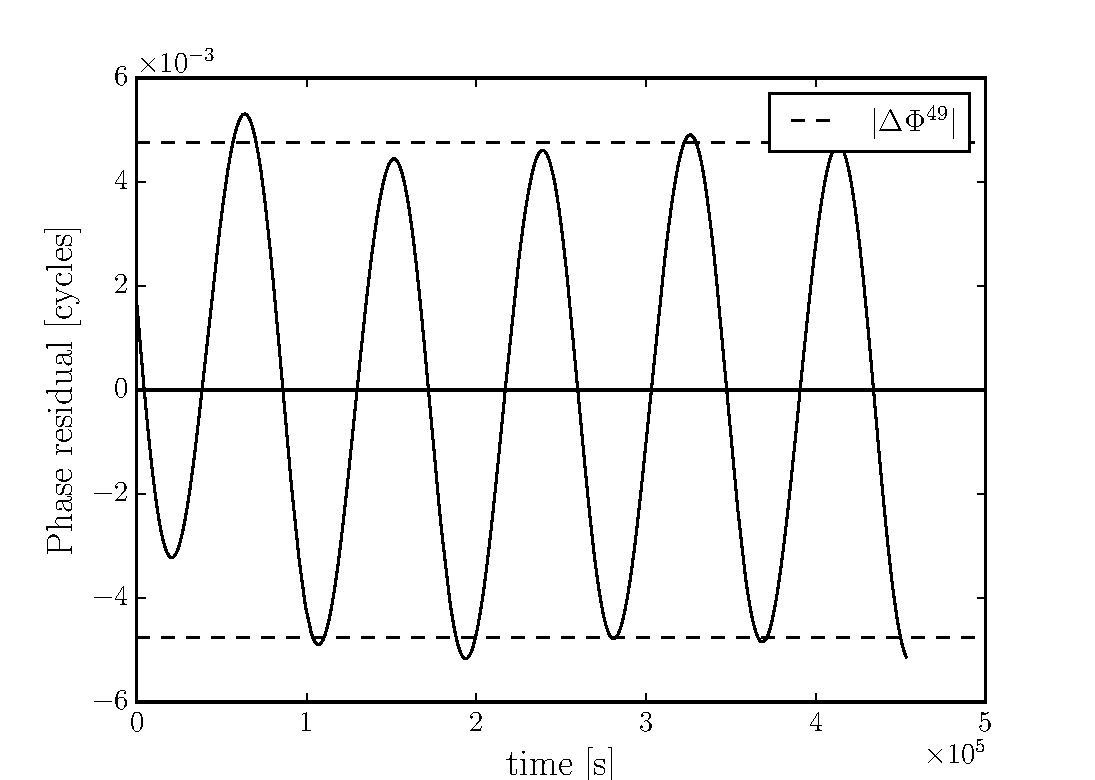
\includegraphics[width=0.7\textwidth]{49_verification.pdf}
%\caption{The phase residual in cycles for a simulated NS with the properties described in table \ref{tab: 49
%verification properties}. This is used to illustrate the agreement with the magnitude
%of variations from equation \eqref{eqn: Jones 49} taken from \citet{Jones2001}.}
%\label{fig: TR 49}
%\end{figure}

\begin{figure}[htb]
\begin{floatrow}
\ffigbox{%
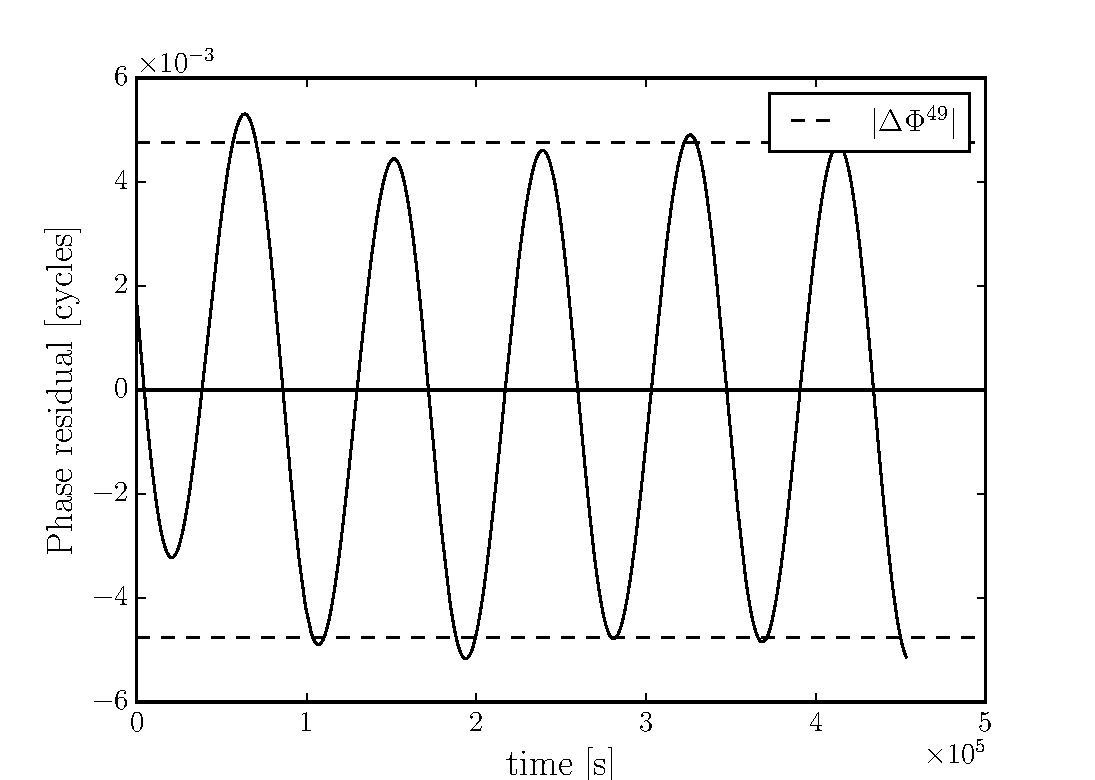
\includegraphics[width=0.5\textwidth]{49_verification.pdf}
}{%
  \caption{The phase residual in cycles for a simulated NS with the properties described in table \ref{tab: 49
verification properties}. This is used to illustrate the agreement with the magnitude
of variations from equation \eqref{eqn: Jones 49} taken from \citet{Jones2001}.}%
  \label{fig: PR 49}
}
\capbtabbox{%
   \begin{tabular}{ccl}
\multicolumn{3}{c}{Simulation parameters} \\
\hline
$\omega_0$  &=& 15.5 rad/s\\
$B_0$  &=& $ 1.581\times 10^{14} $ G \\
$\chi$  &=& 49.99$^{\circ}$ \\
$a_0$ &=& 2.00$^{\circ}$ \\
$\tilde{\theta}$ &= & 2.04$^{\circ}$
\end{tabular}
    
}{%
  \caption{}%
  \label{tab: 49 verification properties}
}
\end{floatrow}
\end{figure}

\FloatBarrier
\subsubsection{Effect of free precession on the phase residual: effect of the 
            electromagnetic torque}
\label{sec: Effect of free precession on the phase residual: effect of the 
            electromagnetic torque}
Considering a vacuum point-dipole spin-down torque (like the one introduced in 
\ref{sec: defining the model}) \citet{Jones2001} found that the EM torque can
amplify the geometric effect of equation \eqref{eqn: Jones 49}. The magnitude
of variation due to EM torque is given by 
\begin{equation}
    |\Delta\Phi^{63}| = \frac{1}{\pi}\left(\frac{\tau_{P}}{P}\right)
    \left(\frac{\tau_{P}}{\tau_{S}}\right) 
                                    |\Delta\Phi^{49}|
\label{eqn: Jones 63}
\end{equation}
The two ratios of time-scales define an `amplification factor':
\begin{equation}
    \mathcal{A}_{\mathrm{EM}} = \left(\frac{\tau_{P}}{P}\right)
                                \left(\frac{\tau_{P}}{\tau_{S}}\right) 
\label{eqn: EM amplification}
\end{equation}
The amplification increases
the magnitude of phase residuals for young pulsars with short periods.

We simulate such a star using the properties in table \ref{tab: 63 verification
properties} noting that the amplification factor is $\sim 3$ when including the
factor of $\pi$. The resulting phase residual is plotted in figure \ref{fig: PR
63} along with the magnitude of variations due to free precession along and the
amplification due to the EM torque. The magnitude of the simulated
phase-residuals are found to agree well with the analytic results of equation
\eqref{eqn: Jones 63}.

%\begin{table}[ht]
%    \centering
%     \begin{tabular}{ccl}
\multicolumn{3}{c}{Simulation parameters} \\
\hline
$\omega_0$  &=& 1550.0 rad/s\\
$B_0$  &=& $ 1.581\times 10^{14} $ G \\
$\chi$  &=& 49.99$^{\circ}$ \\
$a_0$ &=& 2.00$^{\circ}$ \\
$\tilde{\theta}$ &= & 2.06$^{\circ}$ \\
$\mathcal{A}_{\mathrm{EM}}$ &= & $41.0$
\end{tabular}
    
%    \caption{}
%    \label{tab: 63 verification properties}
%\end{table}
%
%\begin{figure}[ht]
%\centering
%	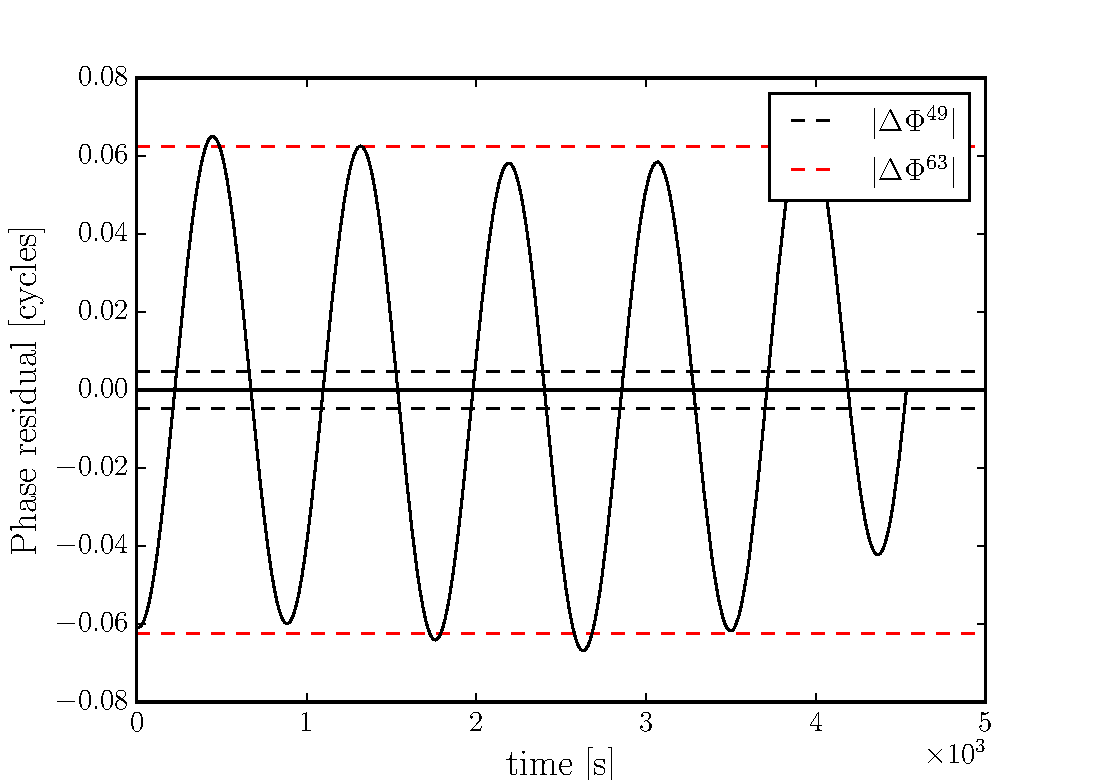
\includegraphics[width=0.7\textwidth]{63_verification.pdf}
%\caption{The phase residual in cycles for a simulated NS with the properties described in table \ref{tab: 49
%verification properties}. This is used to illustrate the agreement with the magnitude
%of variations from equation \eqref{eqn: Jones 49} taken from \citet{Jones2001}.}
%\label{fig: TR 63}
%\end{figure}

\begin{figure}[htb]
\begin{floatrow}
\ffigbox{%
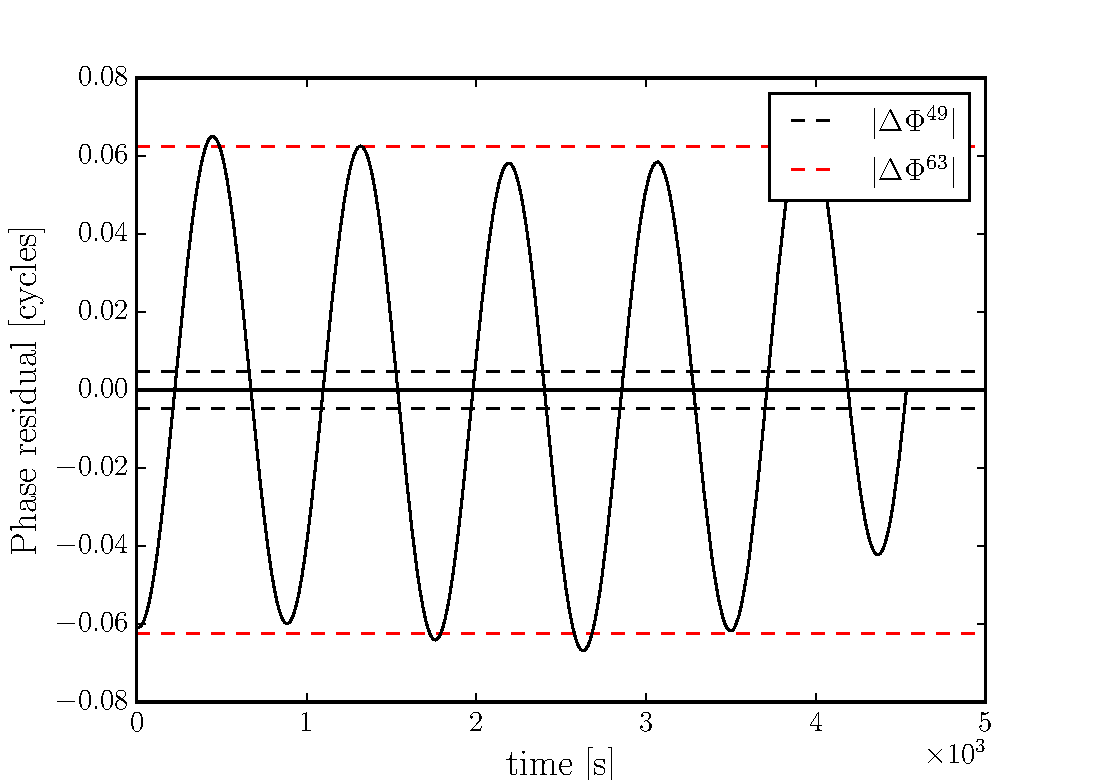
\includegraphics[width=0.5\textwidth]{63_verification.pdf}
}{%
  \caption{The phase residual in cycles for a simulated NS with the properties described in table \ref{tab: 63
verification properties}. This is used to illustrate the agreement with the magnitude
of variations from equation \eqref{eqn: Jones 63} taken from \citet{Jones2001}.}%
  \label{fig: PR 63}
}
\capbtabbox{%
   \begin{tabular}{ccl}
\multicolumn{3}{c}{Simulation parameters} \\
\hline
$\omega_0$  &=& 1550.0 rad/s\\
$B_0$  &=& $ 1.581\times 10^{14} $ G \\
$\chi$  &=& 49.99$^{\circ}$ \\
$a_0$ &=& 2.00$^{\circ}$ \\
$\tilde{\theta}$ &= & 2.06$^{\circ}$ \\
$\mathcal{A}_{\mathrm{EM}}$ &= & $41.0$
\end{tabular}
    
}{%
  \caption{}%
  \label{tab: 63 verification properties}
}
\end{floatrow}
\end{figure}

%In figure \ref{fig: TR no torque} we plot the timing residuals as calculated in
%the torque free model for three values of $\chi$. It is worth noting that the
%power law spin down assumes that the star is in fact spinning down; without the
%torque this model can't not spin down. We can however interpret these results
%as the effect of precession on timing residuals in the limit for which the
%variation due to precession is much stronger than the spin down.
%%\begin{figure}[ht]
%%\centering
%%	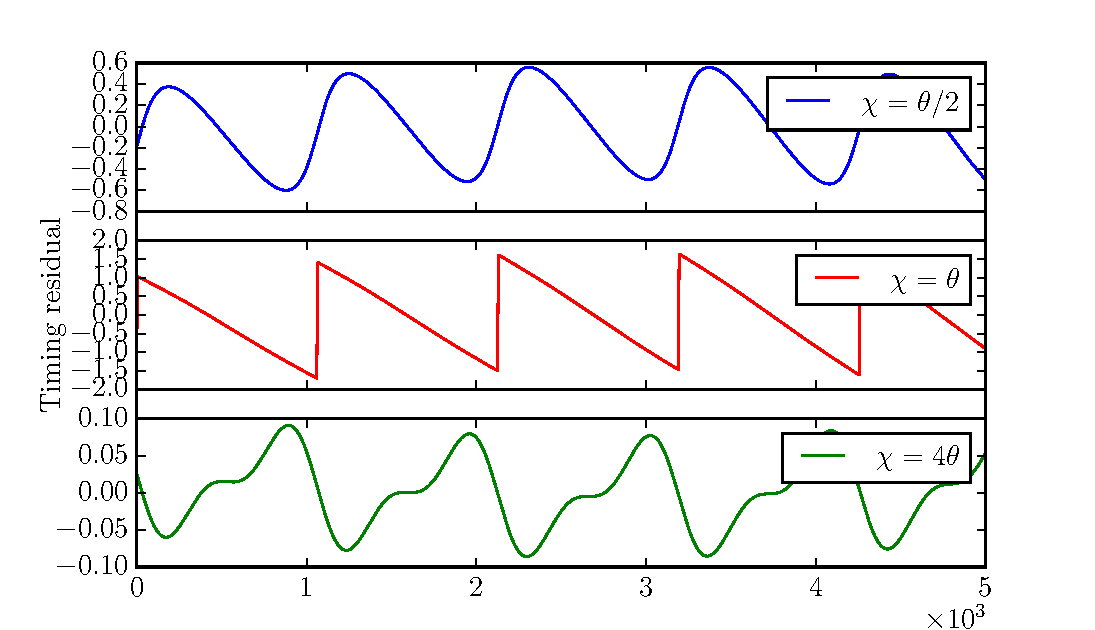
\includegraphics[width=0.7\textwidth]{Timing_residuals_no_torque.pdf}
%%\caption{Plot of the timing residuals for three angles of $\chi$ in the torque
%%         free model showing different types of behaviour. }
%%\label{fig: TR no torque}
%%\end{figure}
%The results show that the precession induces a periodic variation on the
%precession timescale, the magnitude is proportional to the angle $\chi$. We 
%also find the results are dependant on the initial angle $a_{0}$.

\subsubsection{Effect of free precession on phase residuals: orthogonal rotator}

In analysing observations of free precession \citet{Jones2001} applied the
model to PSR B1821-11: a pulsar with a strongly periodic residual that has been
cited as a strong candidate for free precession \citet{Stairs2000}. From the
variations in pulse shape an estimate can be made of the wobble angle
$\wobbleangle \sim 3^{\circ}$. Finding that the amplification factor was
important for this pulsar (it can be calculated to be $\approx 380$), 
\citet{Jones2001} attempted to extract the wobble
angle by inverting \eqref{eqn: Jones 63}. This yields a wobble angle that
disagreed with the estimation from a pulse shape variations. The author
concluded that the strong harmonic periodicity's suggested the dipole was
nearly orthogonal e.g. $\chi \approx \pi/2$.  This required expansions of the
phase modulation resulting in an estimate
\begin{equation}
    |\Delta\Phi^{75}| = \frac{1}{4\pi} \frac{\tau_{P}^{2}}{\tau_{S} P} \theta^{2}
    \label{eqn: Jones 75}
\end{equation}

In figure \ref{fig: PR 75} we simulate the B1828-11 pulsar taking the values
from \citet{Stairs2000} and modifying them to allow the simulation to complete
in a reasonable time. The modification was setup such that the amplification
factor remained the same along with the ratio of timescales. The properties
of the simulation are given in \ref{tab: 75 verification properties}

\begin{figure}[htb]
\begin{floatrow}
\ffigbox{%
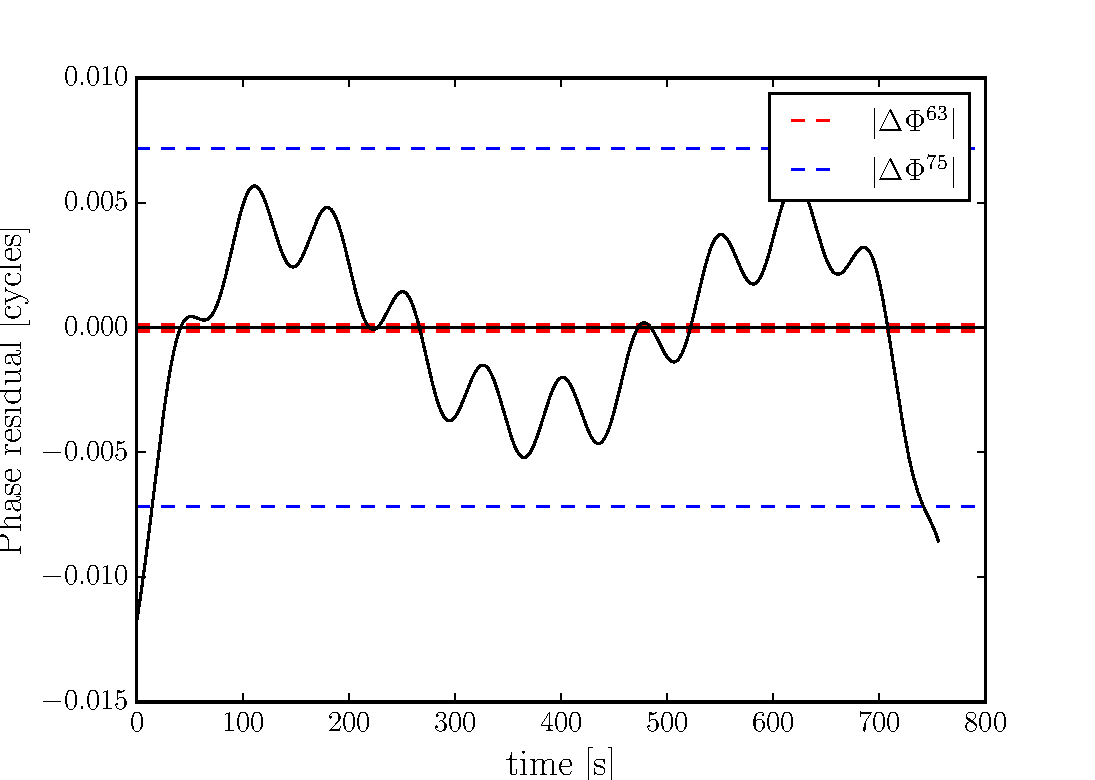
\includegraphics[width=0.5\textwidth]{75_verification.pdf}
}{%
  \caption{The phase residual in cycles for a simulated NS with the properties described in table \ref{tab: 75
verification properties}. This is used to illustrate the agreement with the magnitude
of variations from equation \eqref{eqn: Jones 75} taken from \citet{Jones2001}.}%
  \label{fig: PR 75}
}
\capbtabbox{%
   \begin{tabular}{ccl}
\multicolumn{3}{c}{Simulation parameters} \\
\hline
$\omega_0$  &=& 9310.0 rad/s\\
$B_0$  &=& $ 1.581\times 10^{14} $ G \\
$\chi$  &=& 89.99$^{\circ}$ \\
$a_0$ &=& 2.00$^{\circ}$ \\
$\tilde{\theta}$ &= & 2.11$^{\circ}$ \\
$\mathcal{A}_{\mathrm{EM}}$ &= & $420.0$
\end{tabular}
    
}{%
  \caption{}%
  \label{tab: 75 verification properties}
}
\end{floatrow}
\end{figure}





\FloatBarrier
\subsection{Single torque switching events}
The recent observations by \citet{Lyne2010} suggest that for a few pulsars the
quasi-periodic structure observed in pulsar timing residuals is a result of 
torque-switching events. They find that the spin-down periodically switches
between two distinct values and these changes correlate with changes in the beam
width. They argue this indicates that the electromagnetic torque is periodically
switching between two distinct states. 

We will not discuss where the periodic nature comes from here, but instead
present a direct simulation of the timing residuals from switching events. For
simplicity we begin by consider a single switch in the torque at some time
$t_{\mathrm{switch}}$; for the time being we set this to be half the
observation period, such that $t_{\mathrm{switch}} = \To/2$.

In the EM dipole spindown model the torque has two distinct components: the
regular spin-down part and the so-called anomalous component. This later term 
does not contribute to the spin-down, but as discussed in section \ref{sec: effective
body frame} it will modify the axis of precession. The torque switching will 
occur in the spin-down component, but it seems unlikely that it will also
occur in the anomalous component [Ian - why?]. To cover all cases we 
model a single torque switching effect by redefining the torque in equation
\eqref{eqn: torque} such that

\newcommand{\Ss}{S_{\mathrm{S}}}
\newcommand{\Sa}{S_{\mathrm{A}}}

\begin{equation}
\mathbf{T} = (1 - \Ss H(t-t_{\mathrm{switch}})) \mathbf{T}_{\mathrm{S}}+
                 (1 - \Sa H(t-t_{\mathrm{switch}})) \mathbf{T}_{\mathrm{A}}
\label{eqn: single switch torque}
\end{equation} 
where the subscripts label the spin-down and anomalous components, $S$ is the
strength of switching, and $H(t)$ is the Heaviside function. 

Numerically solving the body-frame and Euler equations using this torque we 
simulate a single switching event to try and understand the effect it will have
on phase residuals. 

\subsubsection{Minimal precession}
Without the torque-switching, in these simulations only free precession can 
produce structure in the phase residuals. No pulsars exist with regular periodic
structure that can be solely interpreted as free precession. Most pulsars must 
therefore exist with very small wobble angles with any excitement of this being
damped. As such, we begin by discussing the "minimal precession" initial 
conditions from which to start our simulations. 


Precession will not occur when the spin vector is aligned with the axis about
which it rotates. The angle between these two we have defined as the wobble
angle.  For minimal precession we should therefore set this wobble angle to
zero. In all simulations we consider a biaxial body with the full torque given
in \eqref{eqn: single switch torque}. From our previous discussion on the 
wobble angle we can minimise the precession by setting the initial polar angle
of the spin vector in the body frame to lie along the effective body-frame 
axis. That is
\begin{equation}
a_{0} = \beta(\epsI, \epsA, \chi),
\end{equation}
we refer to such a simulation as `minimal precession' since the wobble angle 
remains non-zero.

In this case the wobble angle will given by equation \eqref{eqn: spindown wobble angle}:
The magnitude of variations in the phase-residuals is given by inserting this
wobble angle
\begin{equation}
\wobbleangle \approx \frac{1}{\epsI}{\frac{P}{\tauS}}
\end{equation} 
into either equation \eqref{eqn: Jones 45} or \eqref{eqn: Jones 75} depending 
on the EM amplification factor.

We verify this by setting up a minimal precession simulation. The resulting
phase residual is given in figure \ref{fig: no switching} along with the
predicted magnitude of variations. In table \ref{tab: NoSwitching properties}
we give the simulation properties: note that the initial polar angle is exactly
the angle $\beta$ which can be calculated using equation \eqref{eqn: beta}. 
The wobble angle is given by equation \eqref{eqn: wobble angle} and is non-zero
due to the spindown torque. 

\begin{figure}[htb]
\begin{floatrow}
\ffigbox{%
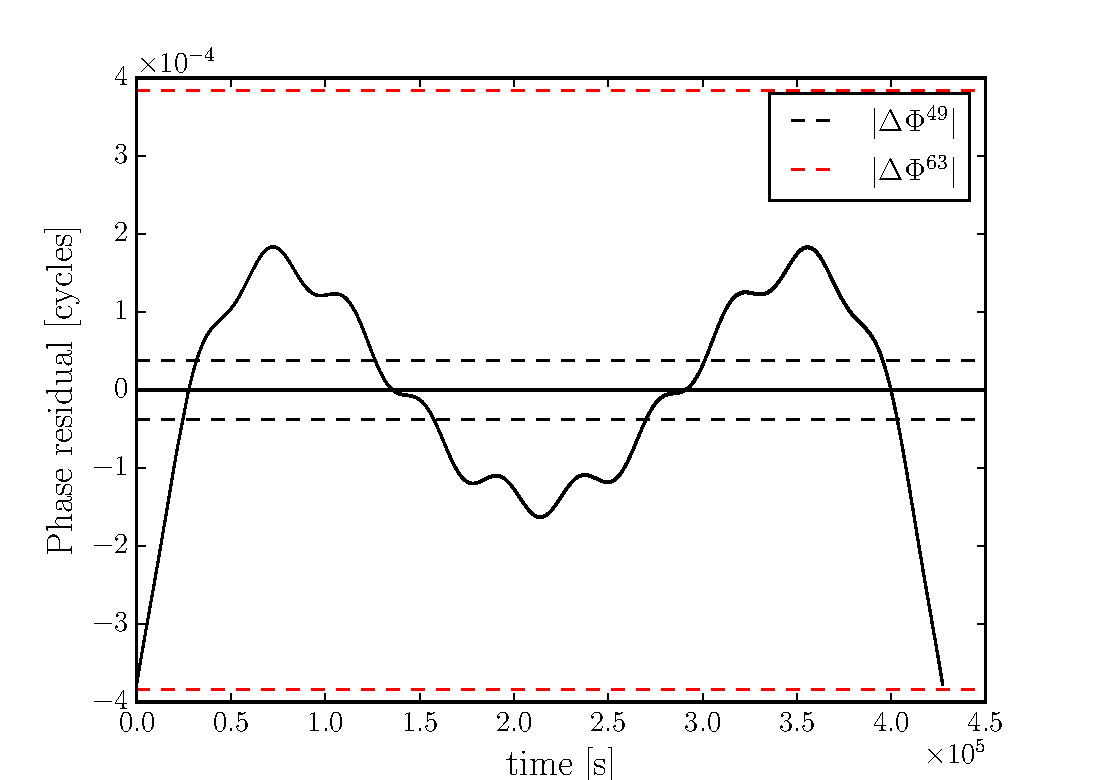
\includegraphics[width=0.5\textwidth]{NoSwitching.pdf}
}{%
    \caption{}
  \label{fig: no switching}
}
\capbtabbox{%
   \begin{tabular}{ccl}
\multicolumn{3}{c}{Simulation parameters} \\
\hline
$\omega_0$  &=& 15.0 rad/s\\
$B_0$  &=& $ 2.683\times 10^{15} $ G \\
$\chi$  &=& 60.10$^{\circ}$ \\
$a_0$ &=& -4.46$^{\circ}$ \\
$\tilde{\theta}$ &= & 0.02$^{\circ}$ \\
$\mathcal{A}_{\mathrm{EM}}$ &= & $31.0$
\end{tabular}
    
}{%
  \caption{}%
  \label{tab: NoSwitching properties}
}
\end{floatrow}
\end{figure}


We will now setup a simulation of this `minimal precession` NS, and then 
manually switch the torque. We choose a NS where the EM torque amplification
given in equation \eqref{eqn: Jones 75} is important.

\FloatBarrier
\subsection{Switching without the anomalous torque}
We now consider manually switching the spindown torque halfway though the simulation.
That is we set
\begin{align}
    t_{\mathrm{switch}} = \frac{\To}{2}, &&& \Ss = 0.4, &&& \Sa = 0.0,
\end{align}
such that halfway though the simulation the spindown torque is reduced by a
fraction $0.4$ while the anomalous torque remains unaffected. 

In figure \ref{fig: switching without anom} we plot the phase residuals from
this simulation. In the top plot is the residual as calculated over the entire
observation period. We find a single periodic variation with significantly
larger variation than any of the precession features. This is a direct result
of the switching only as discussed in section \ref{sec: Lyne two state}: the
effect of precession is entirely swamped by the switching. For this reason in
the lower plot we calculate two residuals: the first is calculated
in the region $[0, t_{\mathrm{switch}}]$ and the second in $[t_{\mathrm{switch}}, \To]$.
Because the switch does not occur in either of these periods we can resolve the
free precession during each period.

\begin{figure}[htb]
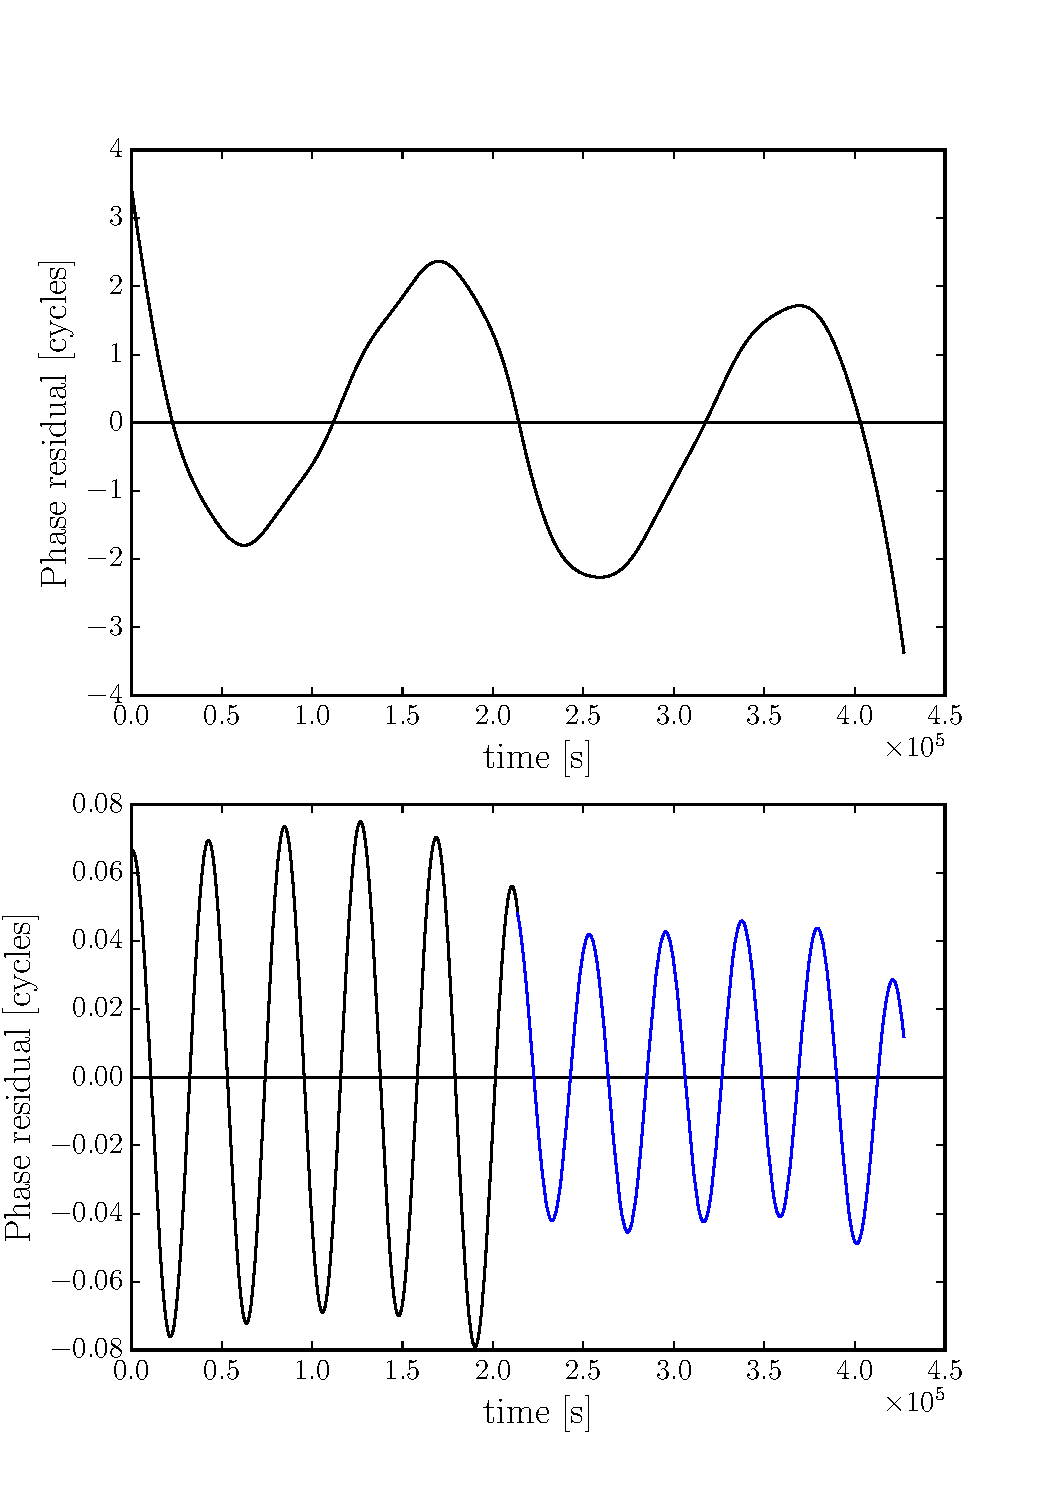
\includegraphics[width=.5\textwidth]{SwitchingWithoutAnomTorque}
\caption{}
\label{fig: switching without anom}
\end{figure}

The simulations begin in the minimal precession state where the spin-vector
is aligned with the effective body frame axis such that the wobble angle is given
by equation \eqref{eqn: spindown wobble angle}. After the switch, the wobble
angle is smaller by a factor $\Ss$ and as a result we see the precession is
reduced by this fraction.


\FloatBarrier
\subsection{Switching with the anomalous torque}
We now consider manually switching both the spindown and anomalous torque
halfway though the simulation.  That is we set
\begin{align}
    t_{\mathrm{switch}} = \frac{\To}{2}, &&& \Ss = \Sa = 0.01
\end{align}

In a similar fashion to figure \ref{fig: switching without anom} we show first
the total residual in the top plot of figure \ref{fig: switching with anom}, and
then the individual residuals in the lower plot.

In this simulation we have used a significantly smaller switching fraction 
than when switching without the anomalous torque. This is because the effect 
on the phase residuals when calculated in the two regions is significantly
stronger. This is because we begin with a `minimal precession' state, where
$\theta = \beta$ and the precession results from effect of the spin-down torque.
Then, when we switching off a fraction of the anomalous torque we have modified
the effective body frame and hence the angle $\beta$. This generates a significantly
larger wobble angle producing a significant increase in the phase residuals
fitted in the post-switch period. The effect is not observable when fitting
to the entire simulation period since the switching event remains dominant.

\begin{figure}[htb]
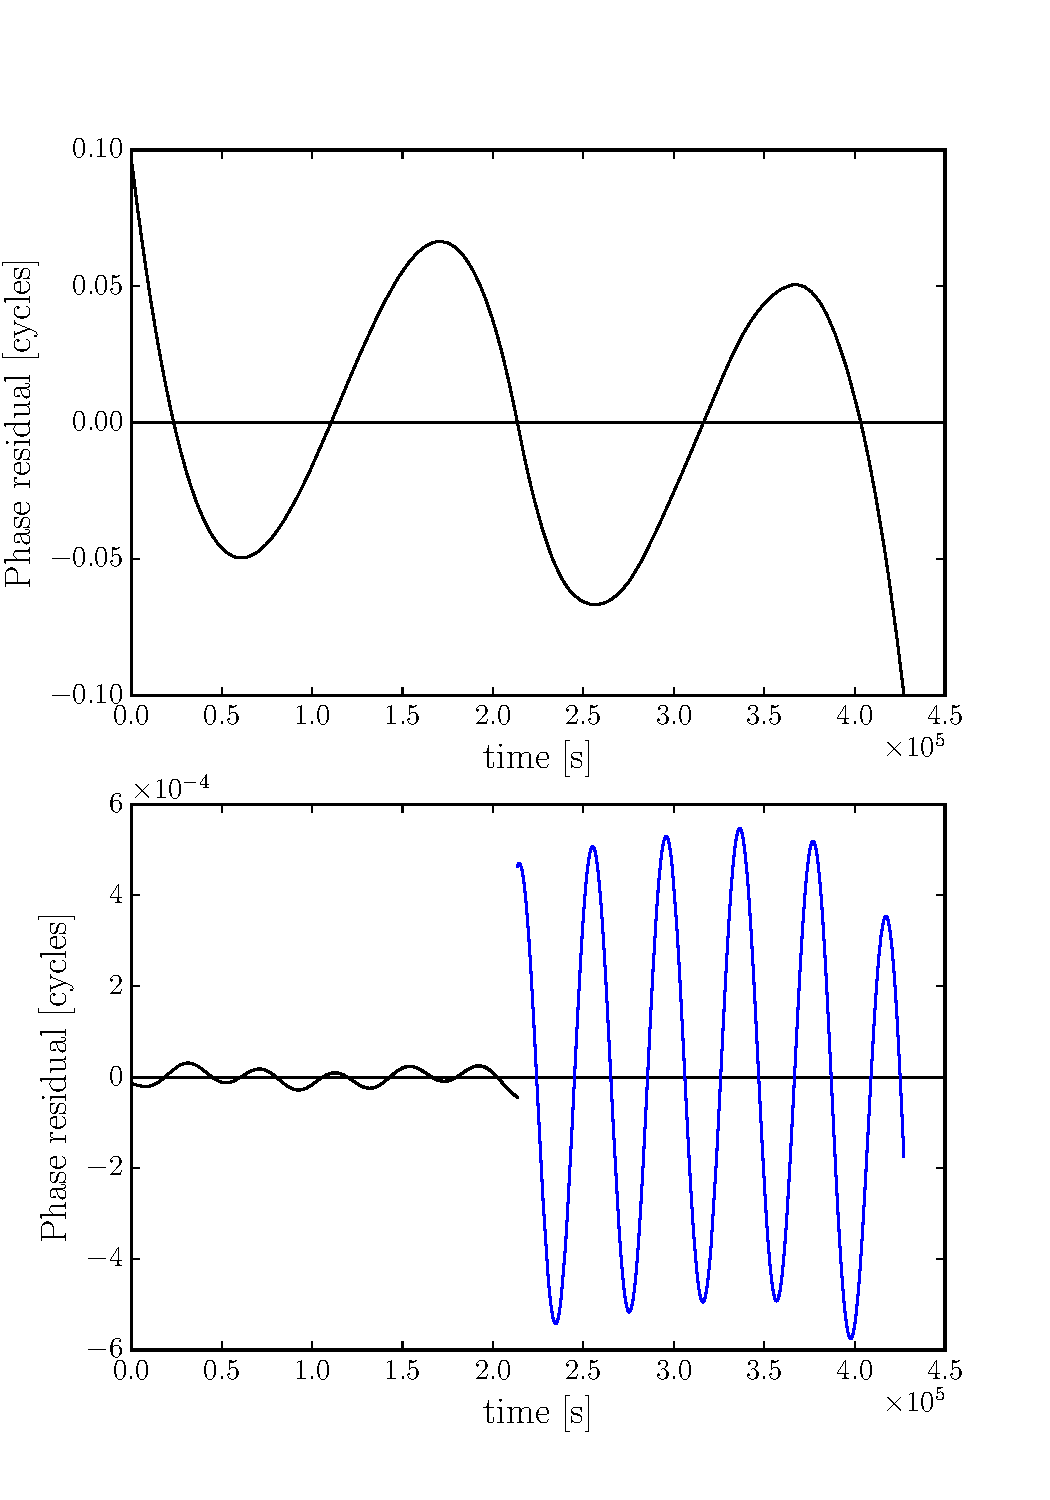
\includegraphics[width=.5\textwidth]{SwitchingWithAnomTorque}
\caption{}
\label{fig: switching with anom}
\end{figure}




\biblio
\end{document}

